
\chapter{Arhitektura i dizajn sustava}



Arhitektura sustava je struktura sustava koja sadrži: elemente programa, njihove izvana vidljive karakteristike te odnose među njima.
Arhitektura sustava se dijeli na tri manja sustava:
\begin{packed_item}
	\item[$\bullet$] Web preglednik
	\item[$\bullet$] Web aplikacija
	\item[$\bullet$] Baza podataka
\end{packed_item}



\underbar {\textit {Web preglednik}} je program preko kojega korisnik može pregledavati web-stranice te multimedijalne sadržaje od tih web-stranica. Web-stranica je napisana u kodu koji web preglednik prevodi tako da svatko razumije web-stranicu. Web preglednik također služi kao kanal između korisnika i web poslužitelja.


\underbar {\textit {Web poslužitelj}} služi za komunikaciju između klijenta i aplikacije. Ta komunikacija se odvija preko HTTP-a. HTTP je protokol koji se koristi za prijenos podataka na webu. Web poslužitelj također pokreće web aplikaciju i prosljeđuje joj zahtjeve.


\underbar {\textit {Web aplikacija}} obrađuje zahtjeve od korisnika, a za pojedine zahtjeve ona pristupa bazi podataka nakon čega se odgovor šalje korisniku putem web poslužitelja te web preglednika u HTML obliku.


\begin{figure}[H]
	\centering
	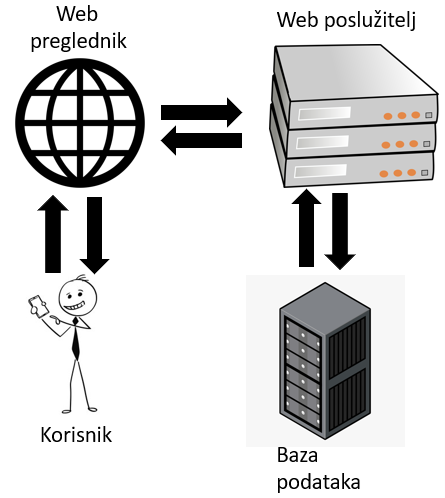
\includegraphics[width=0.75\textwidth]{slike/arhitektura_sustava.PNG} 
	\caption{Arhitektura sustava}
	\label{fig:promjene1} 
\end{figure}


U našemu sustavu za razvoj radnog okvira na poslužiteljskoj strani (backend-u) odlučili smo koristiti \textit {Spring Boot}, a na klijentskoj strani (frontend-u) smo odlučili koristiti \textit {React}. Programske jezike za koje smo se odlučili su \textit {Java} i \textit {JavaScript}.


Korišteni razvojni okvir Spring se služi tzv. MVC arhitekturom. Takva arhitektura podrazumijeva sljedeću podjelu:
\begin{itemize}
	\item[$\bullet$] \textbf{Model}: Središnja komponenta sustava, dohvat te manipulacija podataka
	\item[$\bullet$] \textbf{View}: dostupni razni prikazi podataka (tablično, grafom)
	\item[$\bullet$] \textbf{Controller}: upravlja zahtjevima korisnika te na temelju njih izvodi daljnju interakciju s ostalim komponentama
\end{itemize}

\vspace{3cm}

Naša web aplikacija koristi višeslojni stil arhitekture. Prednosti višeslojnog stila arhitekture su brojne:

\begin{packed_item}
	\item[$\bullet$] olakšava razvoj programa
	\item[$\bullet$] timovi se mogu raspodijeliti na razvoj zasebnih slojeva arhitekture
	\item[$\bullet$] podjela briga odnosno svaki sloj se mora brinuti za samo svoju zadaću
	\item[$\bullet$] moguće je jednostavno povećanje i poboljšanje sustava
\end{packed_item}







\section{Baza podataka}




\subsection{Vrsta i implementacija}
Za modeliranje sustava je korištena relacijska baza podataka, a nju smo implementirati pomoću open-source sustava za upravljanje bazama podataka PostgreSQL. Za izradu dijagrama ER i generiranje relacijske sheme je korišten besplatan online alat ERDplus (https://erdplus.com/) koji je korišten i u sklopu predmeta Baze podataka. 



\subsection{Glavne komponente baze podataka}
Baza podataka sastoji se od sljedećih entiteta:

\begin{itemize}
	\item \textbf{User} \hspace{0.15cm} (\textit{id}, \textit{email} \textit{username}, \textit{password}, \textit{name}, \textit{lastName}, \textit{IBAN}, \textit{photo}, \textit{role}, \textit{walletBalance}, \textit{approved}, \textit{verified}, \textit{verificationToken})
	
	
	\item \textbf{Parking} (\textit{picture}, \textit{parkingName}, \textit{parkingDescription}, \textit{costPerHour}, \textit{parkingId}, \textit{voditeljId}) 
	
	\item \textbf{ParkingSpot} (\textit{parkingSpotId}, \textit{latitude}, \textit{longitude}, \textit{polygon}, \textit{label}, \textit{reserveable}, \textit{parkingId})
	
	\item \textbf{Voditelj} (\textit{voditeljId})
	
	\item \textbf{Reservation} (\textit{reservationId}, \textit{duration}, \textit{reservationStart}, \textit{reservationEnd}, \textit{korisnikId}, \textit{parkingSpotId})
	
	\item \textbf{BicycleParking} (\textit{bicycleId}, \textit{latitude}, \textit{longitude}, \textit{numberOfSpots}, \textit{polygon}, \textit{parkingId})
\end{itemize}



\subsection{Opis tablica}





\textbf{User:} sadržava sve bitne informacije o registriranim korisnicima u sustavu. Sadrži atribute: id, email, username, password, name, lastName, IBAN, photo, role, walletBalance, approved, verified, verificationToken. Također sadrži dodatne atribute putem kojih pratimo je li korisnik verificirao e-mail (verified) te, u slučaju
role=voditelj, je li potvrđen od strane administratora (approved).
Ovaj entitet je preko korisničkog identifikatora u One-to-Many vezi s entitetom Rezervacija i u One-to-One vezi s entitetom Voditelj.

\begin{longtblr}[
	label=none,
	entry=none,
	]{
		width = \textwidth,
		colspec={|X[9,l]|X[5,l]|X[20, l]|},
		rowhead = 1,
	}
	\hline \SetCell[c=3]{c}{\textbf{User}} \\ \hline[3pt]	
	\SetCell{LightGreen} id & INT & Jedinstveno korisničko ime \\ \hline
	email & VARCHAR & Email korisnika\\ \hline
	username & VARCHAR & Korisničko ime\\ \hline
	password & VARCHAR & Hash lozinke dobiven s Bcrypt encoderom\\ \hline
	name & VARCHAR & Ime korisnika\\ \hline
	lastName & VARCHAR & Prezime korisnika\\ \hline
	IBAN & VARCHAR &  IBAN korisnika\\ \hline
	photo & BYTEA & Byte array slike osobne iskaznice\\ \hline
	role & INT & Enum koji označava ulogu korisnika ('klijent', 'voditelj', 'administrator')\\ \hline
	walletBalance & NUMERIC & Decimalni broj koji označava koliko novaca se nalazi u novčaniku \\ \hline
	approved & BOOLEAN & Označava je li voditelj potvrđen od strane admina. \\ \hline
	verified & BOOLEAN & Je li korisnik verificiran preko emaila? \\ \hline
	verificationToken & BOOLEAN & Token verifikacije \\ \hline
	
\end{longtblr}



\noindent\textbf{Parking:} Parking: sadrži ključne informacije o parkiralištima. Sadrži atribute koje postavlja voditelj parkirališta: fotografija, naziv, opis i cijena po satu. Uz to sadrži i generiran ID parkirališta. Ovaj entitet je u vezi Many-to-One s entitetom voditelj putem ID-a voditelja i u One-to-Many vezi s ParkingSpotom preko ID-a parkirališta.
\begin{longtblr}[
	label=none,
	entry=none
	]{
		width = \textwidth,
		colspec={|X[10,l]|X[6, l]|X[20, l]|}, 
		rowhead = 1,
	}
	\hline \SetCell[c=3]{c}{\textbf{Parking}} \\ \hline[3pt]
	\SetCell{LightGreen}parkingId & INT & Jedinstveni identifikator parkirališta\\ \hline
	picture & BYTEA & Slika parkirališta koju voditelj može priložiti\\ \hline
	parkingName & VARCHAR & Naziv parkirališta\\ \hline
	parkingDescription & VARCHAR & Opis parkirališta\\ \hline
	costPerHour & NUMERIC & Cijena po satu koju definira voditelj parkirališta\\ \hline
	\SetCell{LightBlue} voditeljId  & INT & Jedinstveni identifikator voditelja parkirališta \\ \hline
	
\end{longtblr}

\noindent\textbf{ParkingSpot:} ParkingSpot sadrži informacije o pojedinačnim parkirnim mjestima unutar parkirališta. U ovu tablicu ćemo unijeti početne informacije o mjestima za automobile koje smo dobili od Overpass API-ja. Ti atributi su id, centralne koordinate parkirališta (dužina, širina) i poligon. Također sadrži oznaku parkirališnog mjesta, informaciju o dostupnosti i mogućnosti rezervacije mjesta koje postavlja voditelj, te ID parkirališta kojemu pripada. U vezi je Many-to-One s entitetom "Parking" putem ID-a parkirališta i One-to-Many s entitetom Rezervacija putem identifikacije parkirališnog mjesta.

\begin{longtblr}[
	label=none,
	entry=none
	]{
		width = \textwidth,
		colspec={|X[6,l]|X[6, l]|X[20, l]|}, 
		rowhead = 1,
	}
	\hline \SetCell[c=3]{c}{\textbf{ParkingSpot}} \\ \hline[3pt]
	\SetCell{LightGreen}parkingSpotId & VARCHAR & Identifikacija mjesta koje generira overpassAPI koji generira overpassAPI. \newline Npr. "node/11310562209" \\ \hline
	label & VARCHAR & Oznaka ili broj parkirališnog mjesta\\ \hline
	longitude & NUMERICAL & Označuje duljinu  \\ \hline
	latitude & NUMERICAL & Označuje širinu \\ \hline
	reserveable & BOOLEAN & Je li mjesto slobodno ili nije\\ \hline
	polygon & VARCHAR & Poligon parkirališnog mjesta\\ \hline
	\SetCell{LightBlue}parkingId & INT & Jedinstveni identifikator parkirališta \newline (Parking.parkingId)\\ \hline
	
\end{longtblr}

\noindent\textbf{Voditelj:} sadrži informacije o voditeljima parkirališta. Povezuje voditelja sa
parkiralištem. Ima vezu One-to-One s entitetom Korisnik i One-to-Many s Parkingom.
\begin{longtblr}[
	label=none,
	entry=none
	]{
		width = \textwidth,
		colspec={|X[6,l]|X[6, l]|X[20, l]|}, 
		rowhead = 1,
	}
	\hline \SetCell[c=3]{c}{\textbf{Voditelj}} \\ \hline[3pt]
	
	\SetCell{LightGreen}voditeljId & INT & Jedinstveni identifikator voditelja parkirališta \\ \hline
	
\end{longtblr}

\noindent\textbf{Reservation:} sadrži sve rezervacije koje su napravili korisnici. Ovaj entitet
ima vezu Many-to-One s entitetom Korisnik putem korisničkog identifikatora. Također, ima vezu Many-to-One s entitetom ”ParkingSpot” putem lokacije parkirnog mjesta.
\begin{longtblr}[
	label=none,
	entry=none
	]{
		width = \textwidth,
		colspec={|X[9,l]|X[6,l]|X[19, l]|},  % Adjust the width for the second column
		rowhead = 1,
	}
	\hline \SetCell[c=3]{c}{\textbf{Reservation}} \\ \hline[3pt]
	\SetCell{LightGreen}reservationId & INT & Jedistven identifikator rezervacije\\ \hline
	duration & INT & Trajanje rezervacije\\ \hline
	reservationStart & TIMESTAMP & Početak rezervacije \\ \hline
	reservationEnd & TIMESTAMP & Kraj rezervacije\\ \hline
	\SetCell{LightBlue}korisnikId & INT & Jedinstveno korisničko ime\\ \hline
	\SetCell{LightBlue}parkingSpotId & INT & Jedinstven identifikator parkirališnog mjesta \newline \newline\\ \hline
\end{longtblr}

\noindent\textbf{BicycleParking:} sadrži atribute koje dobivamo pozivom overpassAPI-a: (id, koordinate, broj dostupnih mjesta) te identifikator parkirališta kojem pripada. U Many-to-One vezi je s Parkingom preko identifikatora parkirališta.

\begin{longtblr}[
	label=none,
	entry=none
	]{
		width = \textwidth,
		colspec={|X[9,l]|X[6,l]|X[19, l]|},  % Adjust the width for the second column
		rowhead = 1,
	}
	\hline \SetCell[c=3]{c}{\textbf{BicycleParking}} \\ \hline[3pt]
	\SetCell{LightGreen}bicycleId & INT & Jedistven identifikator parkirališnog mjesta za bicikle\\\hline
	numberOfSpots & INT & Broj dostupnih mjesta na parkingu za bicikle\\ \hline
	longitude & NUMERICAL & Označuje duljinu\\ \hline
	latitude & NUMERICAL & Označuje širinu\\ \hline
	polygon & VARCHAR & Poligon parkirališnog mjesta\\ \hline
	\SetCell{LightBlue}parkingId & INT & Jedinstven identifikator parkirališta \\ \hline
	
	
\end{longtblr}

\subsection{Dijagram baze podataka}


\begin{figure}[H]
	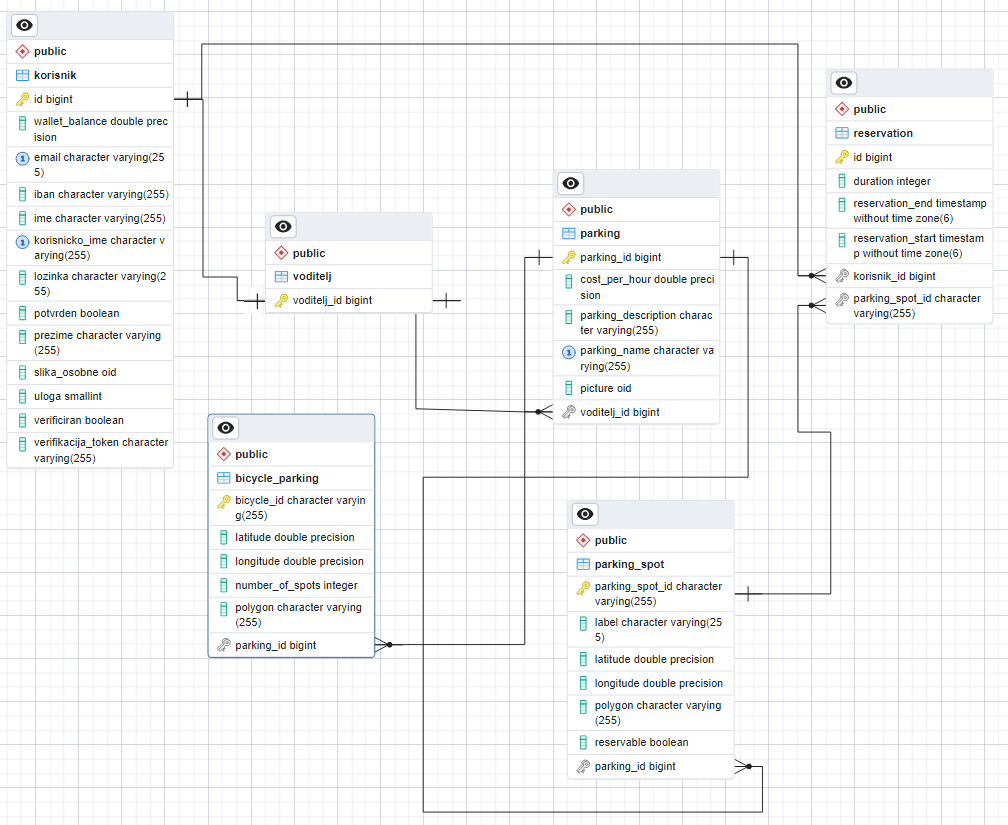
\includegraphics[width=\textwidth]{slike/baza_podataka.png} %veličina slike u odnosu na originalnu datoteku i pozicija slike
	\centering
	\caption{E-R dijagram baze podataka}
	%				\label{fig:dijagramrazreda1}
\end{figure}








\eject


\section{Dijagram razreda}




\begin{figure}[H]
	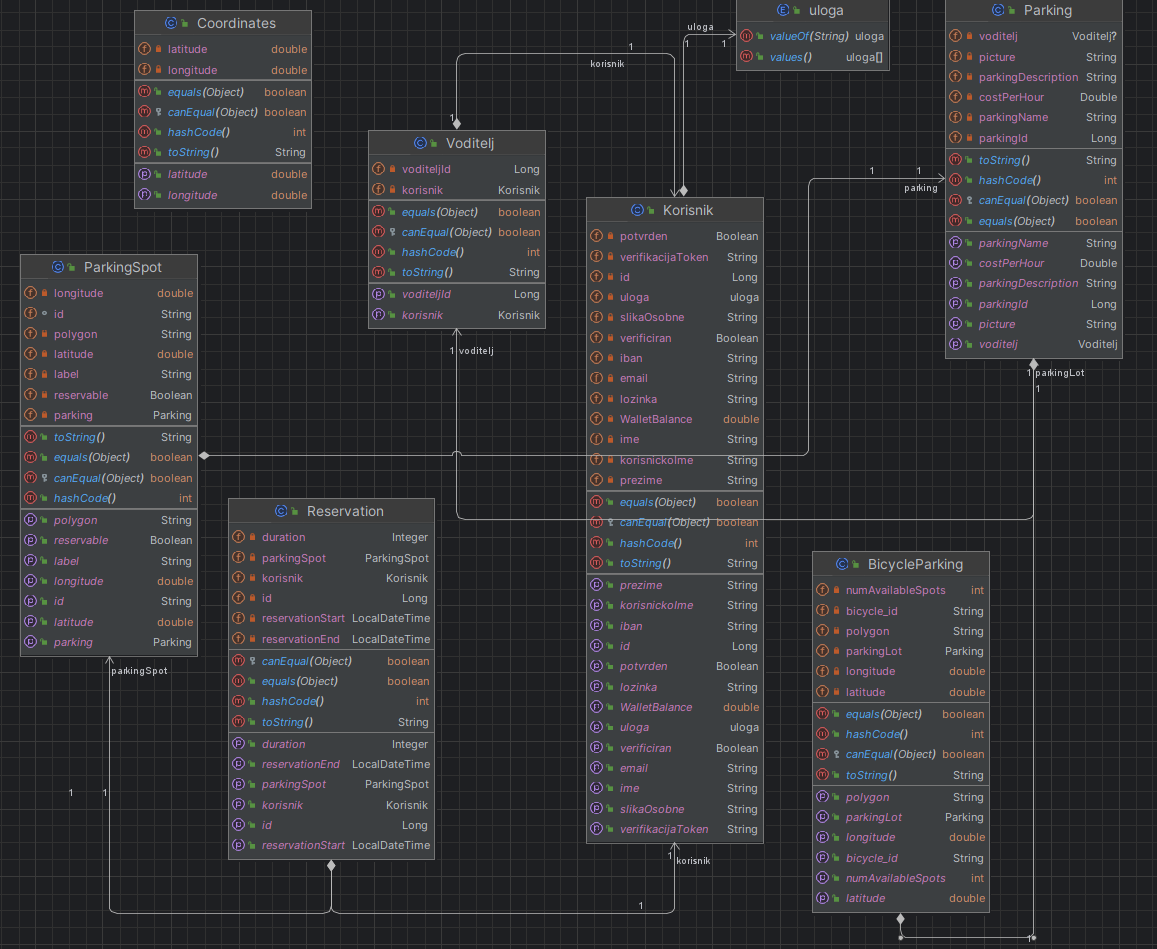
\includegraphics[width=\textwidth]{slike/models.png} %veličina slike u odnosu na originalnu datoteku i pozicija slike
	\centering
	\caption{Dijagram razreda - Modeli}
	%				\label{fig:dijagramrazreda1}
\end{figure}

\begin{figure}[H]
	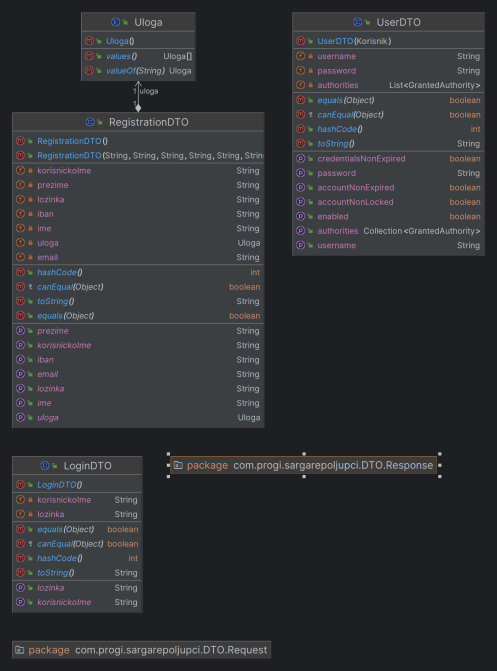
\includegraphics[width=\textwidth]{slike/dto.png} %veličina slike u odnosu na originalnu datoteku i pozicija slike
	\centering
	\caption{Dijagram razreda - Data transfer objects}
	\label{fig:dijagramrazreda2}
\end{figure}




\eject

\section{Dijagram stanja}

UML-dijagram stanja (engl. state machine diagram) je ponašajni UML-dijagram kojim se prikazuje
diskretno ponašanje objekta ili sustava putem prelazaka izmedu konačnog broja stanja.
Ova vrsta dijagrama se koristi za modeliranje ponašanja entiteta tijekom vremena, naglašavajući
odgovor na događaje i okidače. Na slici 4.6 prikazan je dijagram stanja za klijenta, odnosno registriranog korisnika. Nakon prijave, korisniku se prikazuje početna stranica na kojoj može vidjeti vlastite rezervacije. Klijent može pregledavati kartu u stvarnom vremenu te klikom označiti parkirališna mjesta koja ga zanimaju te zatim vidjeti prikaz dostupnih termina za ta parkirališna mjesta. Za klijenta postoji i opcija da prvo odabere termin klikom na odgovarajući termin te zatim bira željena parkirališna mjesta. U slučaju da želi pronaći najbliže parkirališno mjesto, klijent može unijeti odredište, tip vozila i procijenjeno vrijeme trajanja parkinga te će mu aplikacija na karti iscrtati rutu do najbližeg parkirališnog mjesta. Nakon uspješnog plaćanja klijent može vidjeti svoju rezervaciju te ostale rezervacije na početnoj stranici. Klijent u svakom trenutku ima mogućnost pregleda stanja novčanika klikom na "Novčanik" te može po potrebi dodavati sredstva. Klikom na "Osobni podatci" klijent može pregledavati i uređivati osobne podatke ili odabrati opciju brisanja računa.

\begin{figure}[H]
	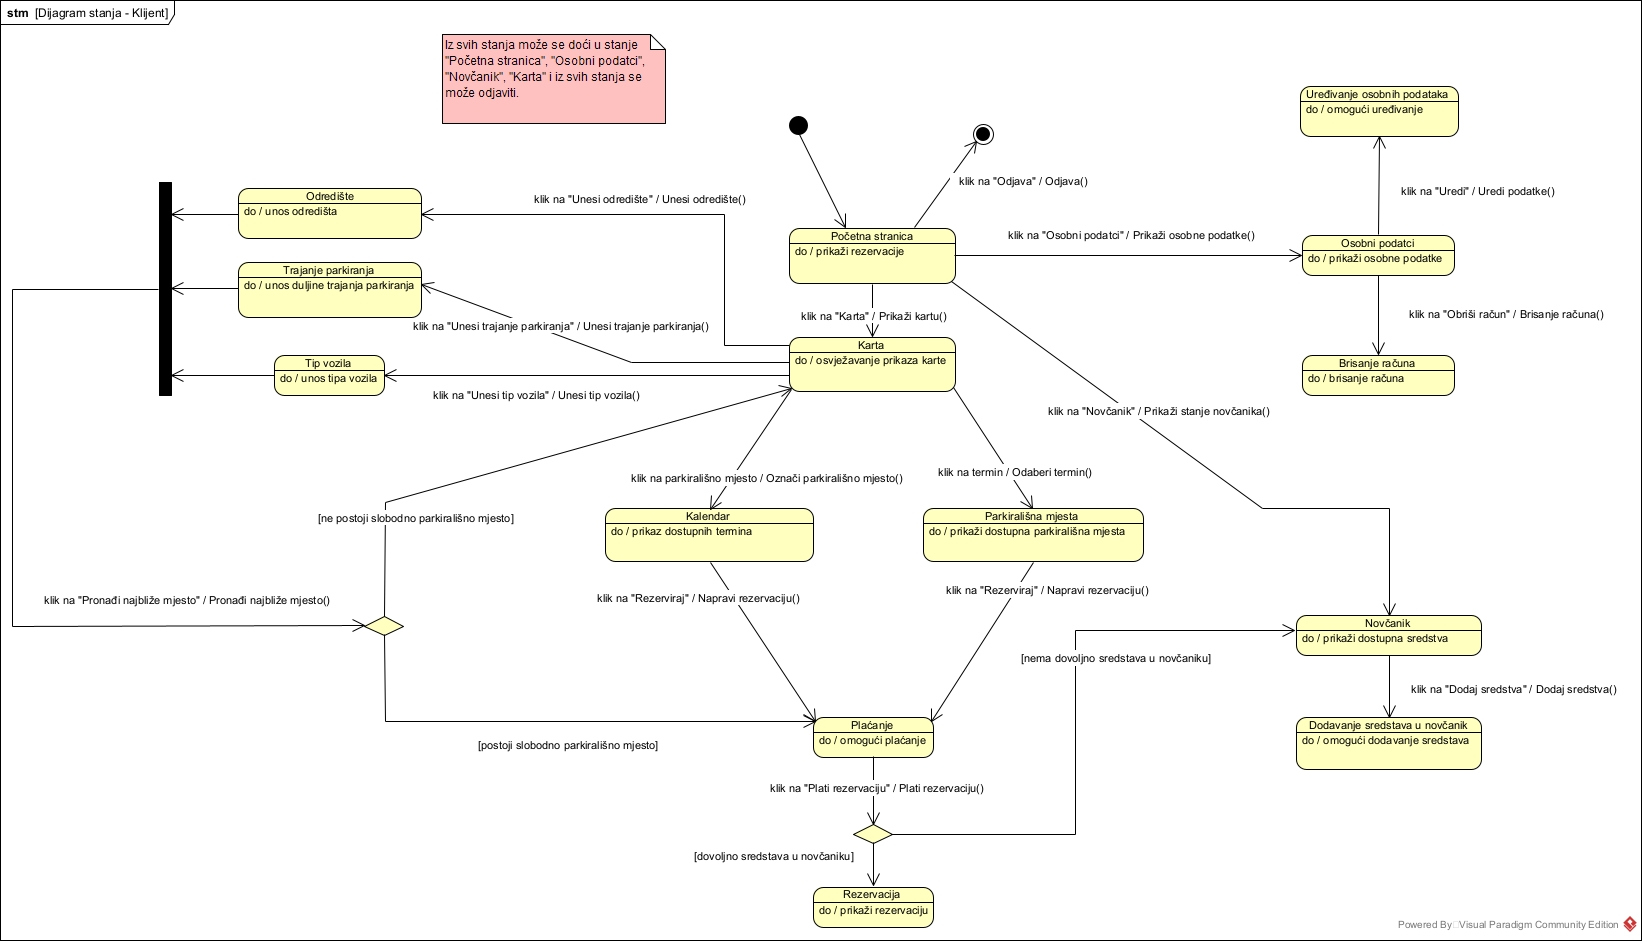
\includegraphics[width=\textwidth]{slike/dijagram_stanja.jpg} %veličina slike u odnosu na originalnu datoteku i pozicija slike
	\centering
	\caption{Dijagram stanja}
	\label{fig:dijagramstanja}
\end{figure}


\eject 

\section{Dijagram aktivnosti}

UML-dijagrami aktivnosti (engl. activity diagrams) su ponašajni UML-dijagrami koji se u programskom inženjerstvu upotrebljavaju za modeliranje i grafički prikaz dinamičkog ponašanja sustava. 
Na njima je prikazano izvođenje aktivnosti kroz niz akcija koje čine upravljačke tokove i tokove objekata. Pokretanje neke akcije uvjetovano je završetkom jedne ili više prethodnih akcija ili dostupnošću objekata i podataka. Registrirani korisnik se prijavljuje u sustav te otvara kartu koja mu prikazuje parkirališna mjesta te informacije o njihovoj zauzetosti. Klijent odabire odredište, tip vozila i trajanje parkinga nakon čega mu aplikacija na karti iscrtava rutu do najbližeg parkirališnog mjesta. Ako je zadovoljan mjestom, klijent stvara i plaća rezervaciju čime ona postaje aktivnom.


\begin{figure}[H]
	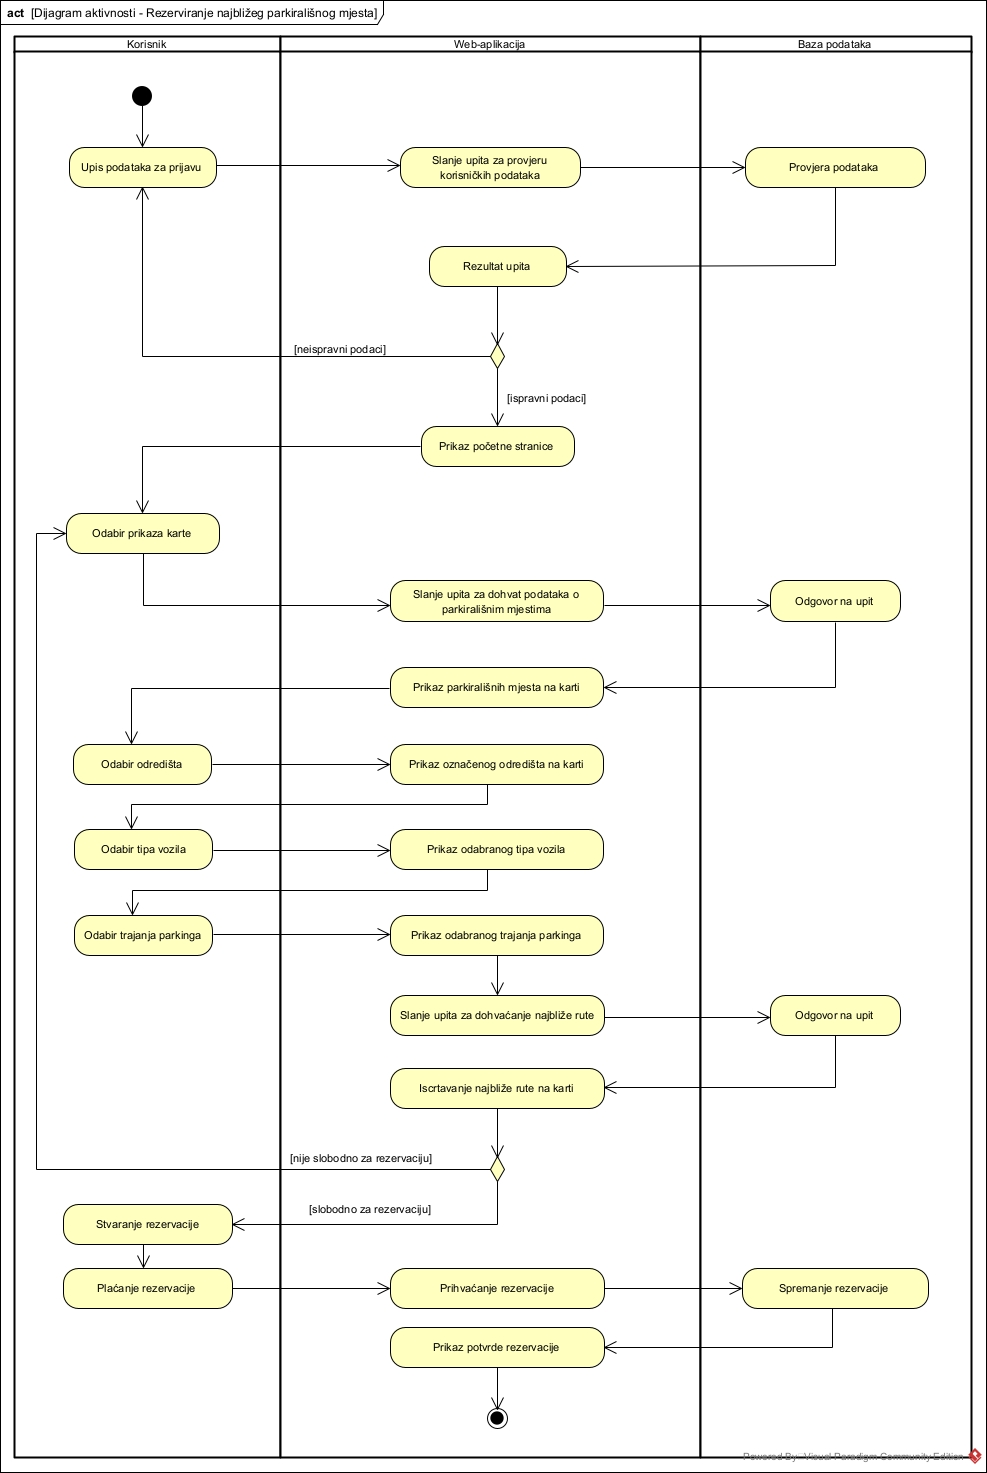
\includegraphics[width=\textwidth, height=\textwidth]{slike/dijagram_aktivnosti.jpg} %veličina slike u odnosu na originalnu datoteku i pozicija slike
	\centering
	\caption{Dijagram aktivnosti}
	\label{fig:dijagramaktivnosti}
\end{figure}


\eject 


\section{Dijagram komponenti}

UML-dijagrami komponenti (engl. component diagrams) su vrsta strukturnih UML-dijagrama koji
prikazuju organizaciju i odnose komponenti koje čine programsku potporu. Pružaju vizualni prikaz 
arhitekture sustava, naglašavajući modularnu strukturu i interakcije između komponenti. Sustavu se pristupa preko
dva različita sučelja. Preko sučelja za dohvat HTML, CSS i JS datoteka poslužuju se 
datoteke koje pripadaju \textit{frontend} dijelu aplikacije. Komponenta \textit{Ruter} na
upit s url određuje koja datoteka će se poslužiti na sučelje, odnosno prikazati korisniku. \textit{Frontend} dio se sastoji od niza JavaScript datoteka koje su raspoređene u logičke cjeline nazvane po tipovima dijelova aplikacije koje prikazuju, odnosno po aktorima koji tim dijelovima aplikacije pristupaju. Sve JavaScript datoteke ovise o React biblioteci iz
koje dohvaćaju gotove komponente kao što su gumbi, forme, stil, obavijesti, tablice, itd. Preko sučelja za dohvat JSON podataka pristupa se Overpass API komponenti. Overpass API poslužuje 
podatke koji pripadaju backend dijelu aplikacije. EF Jezgra zadužena je za dohvaćanje tablica iz baze podataka pomoću SQL upita. Podaci koji su pristigli iz baze se šalju dalje MVC arhitekturi u obliku DTO (Data transfer object).  Web poslužitelj komponenta preko dostupnih sučelja komunicira sa SpotPicker web aplikacijom te ovisno o korisnikovim akcijama osvježava prikaz i dohvaća nove podatke ili datoteke.

\vspace{10cm}

\begin{figure}[H]
	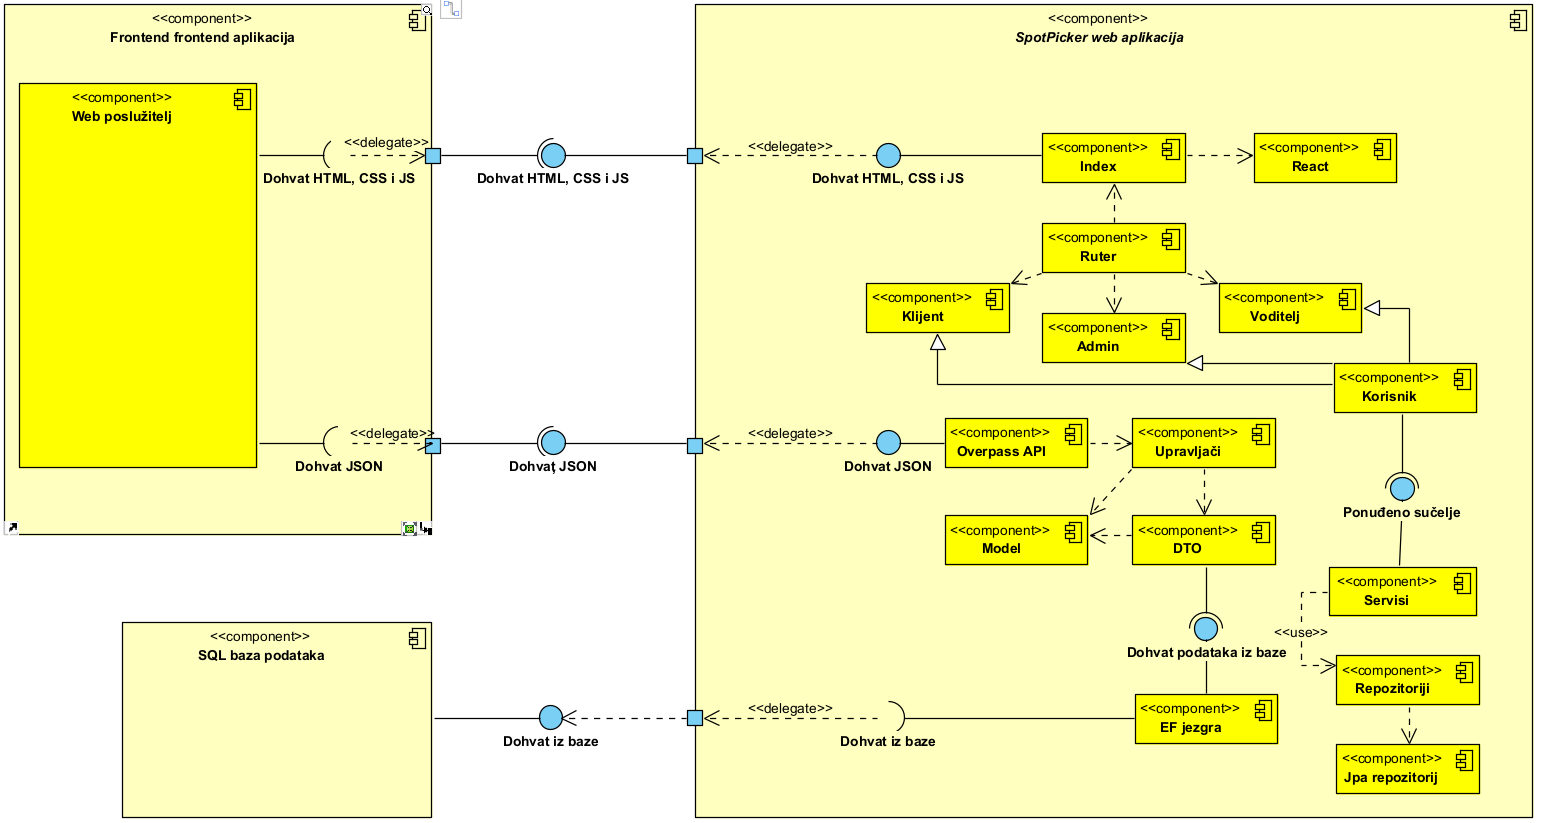
\includegraphics[width=\textwidth]{slike/dijagram_komponenti.png} %veličina slike u odnosu na originalnu datoteku i pozicija slike
	\centering
	\caption{Dijagram komponenti}
	\label{fig:dijagramaktivnosti}
\end{figure}


\eject 

